 \documentclass[%
 aps,
 prl,%
 amsmath,amssymb,
%preprint,%
 reprint,%
%author-year,%
%author-numerical,%
]{revtex4-1}

\usepackage{graphicx}% Include figure files
\usepackage{dcolumn}% Align table columns on decimal point
\usepackage{bm}% bold math
%My packages start
%\usepackage{subfig}
\usepackage{multirow}					
\usepackage{array}
%\usepackage{booktabs}
\usepackage{footnote} 
\newcommand{\angstrom}{\text{\normalfont\AA}}
\usepackage{booktabs}
\usepackage{float}
\usepackage{mathtools}
\usepackage{color}
\newcommand{\comment}[1]{\noindent \textcolor{blue}{#1}}
%My packages end
%\usepackage[mathlines]{lineno}% Enable numbering of text and display math
%\linenumbers\relax % Commence numbering lines

\begin{document}

\title[]{Accelerating atomic structure search with cluster regularization}% Force line breaks with \\

\author{K.\ H.\ S{\o}rensen}
\author{M.\ S.\ J{\o}rgensen ??}
\author{B.\ Hammer}
\email{hammer@phys.au.dk}
\affiliation{ 
Department of Physics and Astronomy, and Interdisciplinary Nanoscience Center (iNANO), Aarhus University, Denmark.
}
% \homepage{phys.au.dk}
 
\date{\today}% It is always \today, today,
             %  but any date may be explicitly specified

\begin{abstract}
\end{abstract}

\pacs{Valid PACS appear here}% PACS, the Physics and Astronomy
                             % Classification Scheme.
\keywords{}%Use showkeys class option if keyword
                              %display desired
\maketitle

\section{\label{sec:introduction}Introduction}
Density functional theory (DFT) has proven successful as the
interaction potential underlying structural searches in computational
materials science. Examples where DFT in combination with experimental information
has provided structural information are abundant in materials science, in particular
for large surface reconstructions, including the SiC(111)-(3$\times$3) surface reconstruction \cite{Starke1998}, the Pd(100)-($\sqrt{5}\times \sqrt{5}$)R27$^o$-O surface oxide \cite{Todorova2003}, the Al$_2$O$_3$/NiAl oxide film \cite{Kresse2005}, and the


\section{Atomic features}
 
The atomic features vectors used in this study is inspried from Botu and Ramprasad \cite{Boto2015} and also used by Xi Chen \cite{Chen2017}.

The length of our feature vector is the number of atomic types plus one. For our system with 2 atomic types the atomic feature vector have length 3.

The first 2 components for each atom $i$, is calculated by finding the list of neighbors $nl(i)$ within a cutoff radius $c$. Then for each of the 2 atomic type T we calculate. 

\begin{equation}
f_T(i) = \sum_{\mathclap{j \in nl(i,c);T=T(j)}} e^{-r_{ij}/1\text{\AA}}f_c(r_{ij})  \label{eq1}
\end{equation}

Here T(j) is the atomic) number of the j'th atom. $r_{ij}$ is the distance from the i'th to the j'th atom in {\AA}ngstr\"{o}m. The last component of the atomic feature vector is $T(i)$ the atomic number for atom i. 
The function $f_c$ make sure that an atoms contribution vanish at the cut-off radius, this gives the gradient higher stability.

\begin{equation}
f_c(r)={{\cos(\pi*r/c)+1}\over 2}
\end{equation}



In figure \ref{fig:fig1} the feature vector is displayed for 1019 structurs of Ti$_{13}$O$_{26}$ with the first component $f_8(i)$ along the x-axis, the second $f_{22}(i)$ along the y-axis and the color is given by the third component $T(i)$. 


\begin{figure}[h]
    \centering
    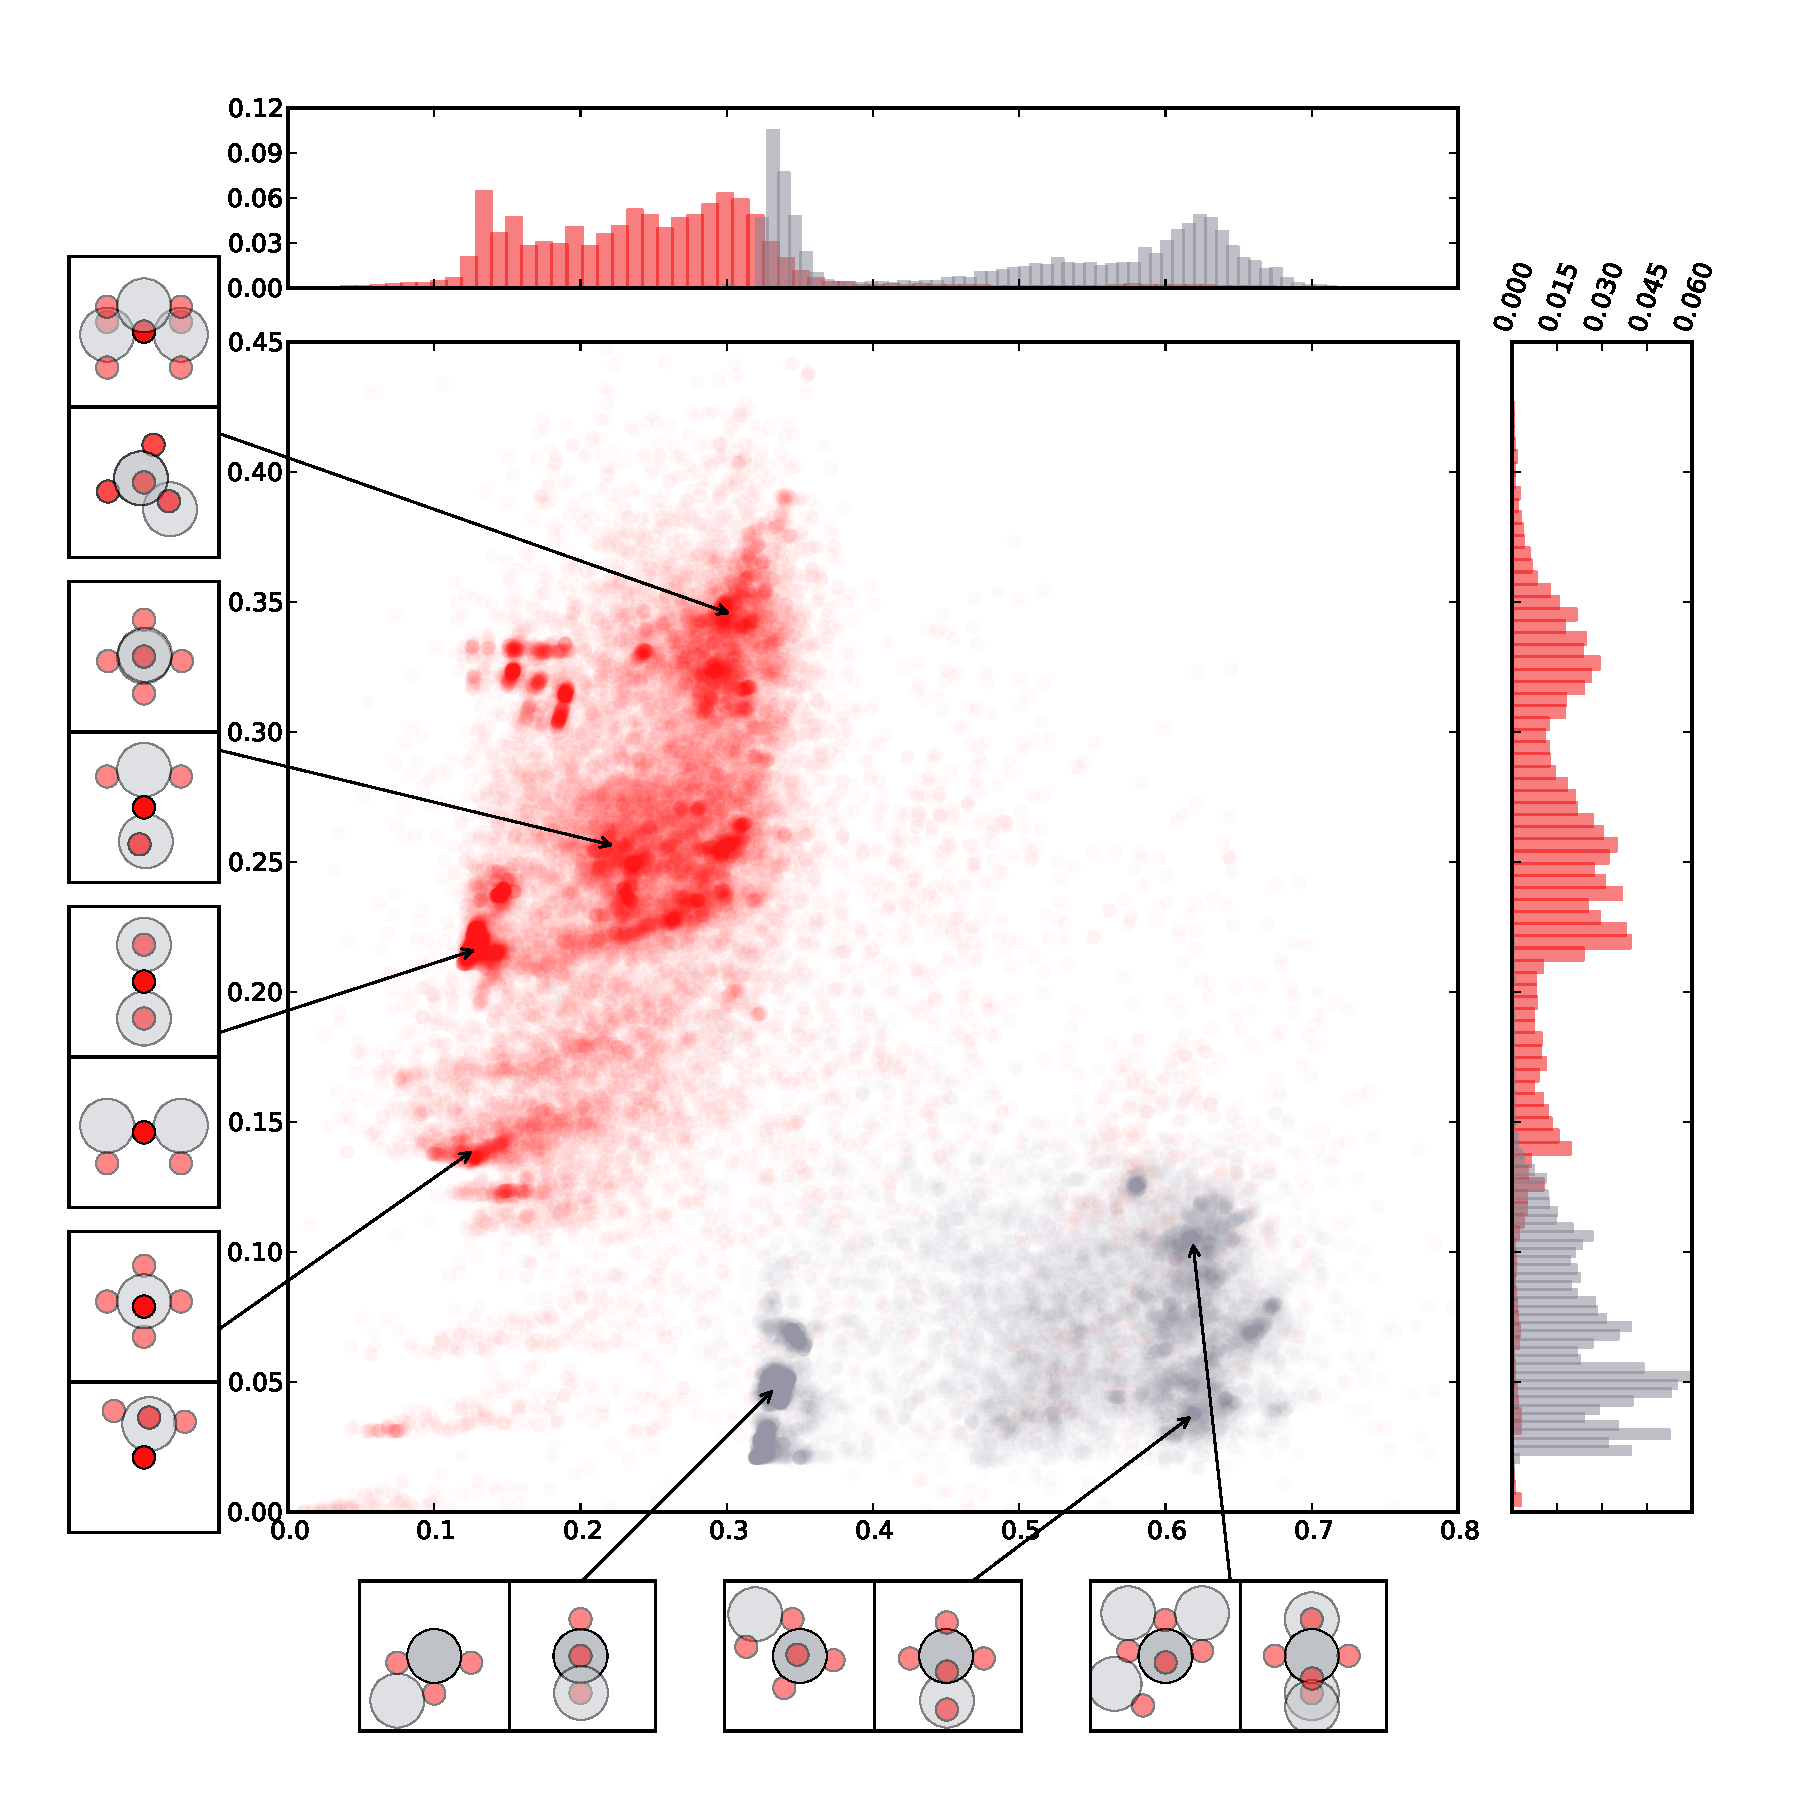
\includegraphics[width=1.0\columnwidth]{ascatter_1_Ti13O26Ridge_1510747669.pdf}
    \caption{Visualization of atoms from 1019 Ti$_{13}$O$_{26}$ structures in feature space}
    \label{fig:fig1}
\end{figure}


\section{Clustering}
The clustering method used is this study is k-means with 2
modifications. The first is a modification to avoid generating empty
clusters \cite{Malay2009} and the second modification is using
k-means++ cluster initialization. While working with clustering on the
atomic feature vectors, the cluster distance vs. energy correlation
illustrated on figure \ref{fig:fig2} was discovered and it was
recognized that it could be applied to speed up minimum energy structure search.   



\begin{figure}[h]
    \centering
    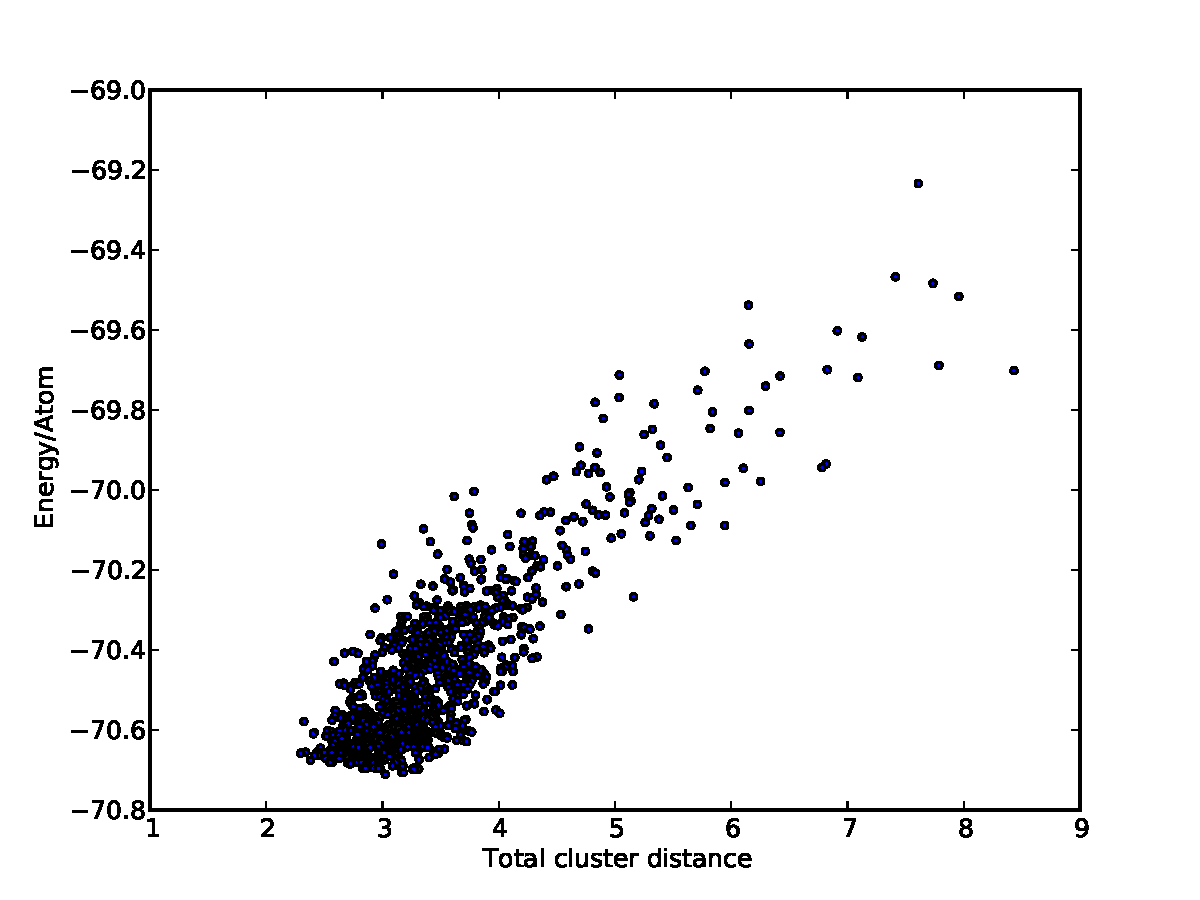
\includegraphics[width=1.0\columnwidth]{decoorL2_5_fgen_Ti13O26Ridge_9_11_9_1510066208.pdf}
    \caption{Cluster distance vs. energy correlation}
    \label{fig:fig2}
\end{figure}




\begin{figure}[h]
    \centering
    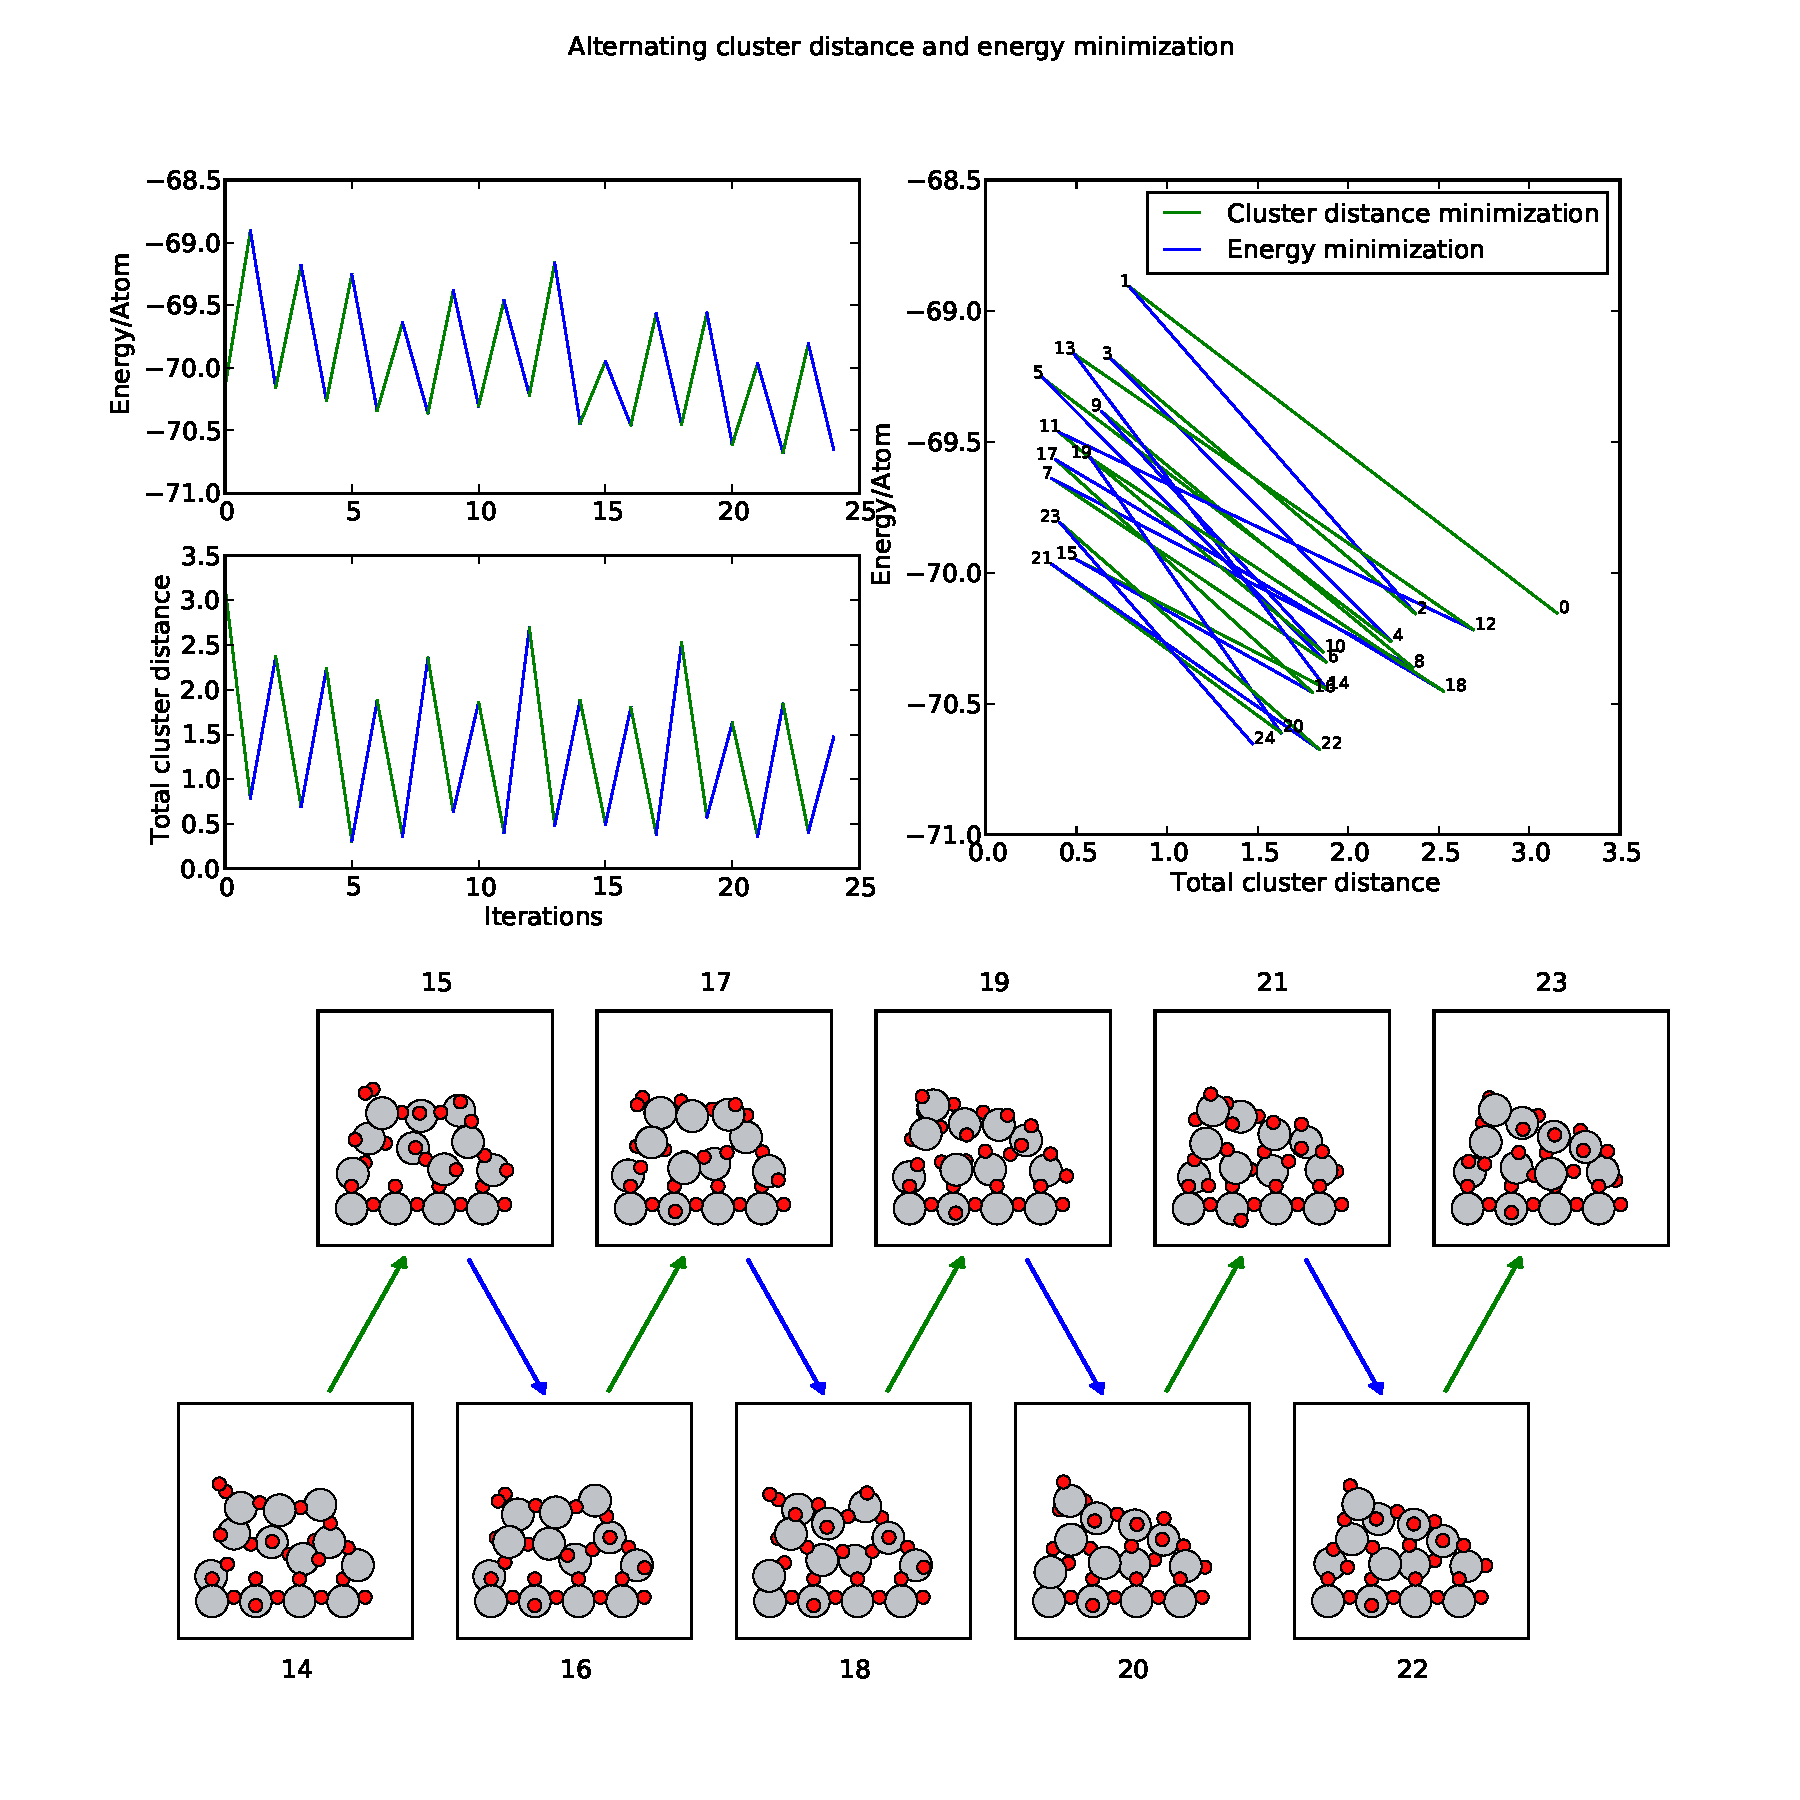
\includegraphics[width=2.0\columnwidth]{acdminplot_74_98_ridgemin2_5_9_500_Ti13O26Ridge.pdf}
    \caption{Combined minimization}
    \label{fig:fig3}
\end{figure}


\section{Search results}

\begin{figure}[h]
    \centering
    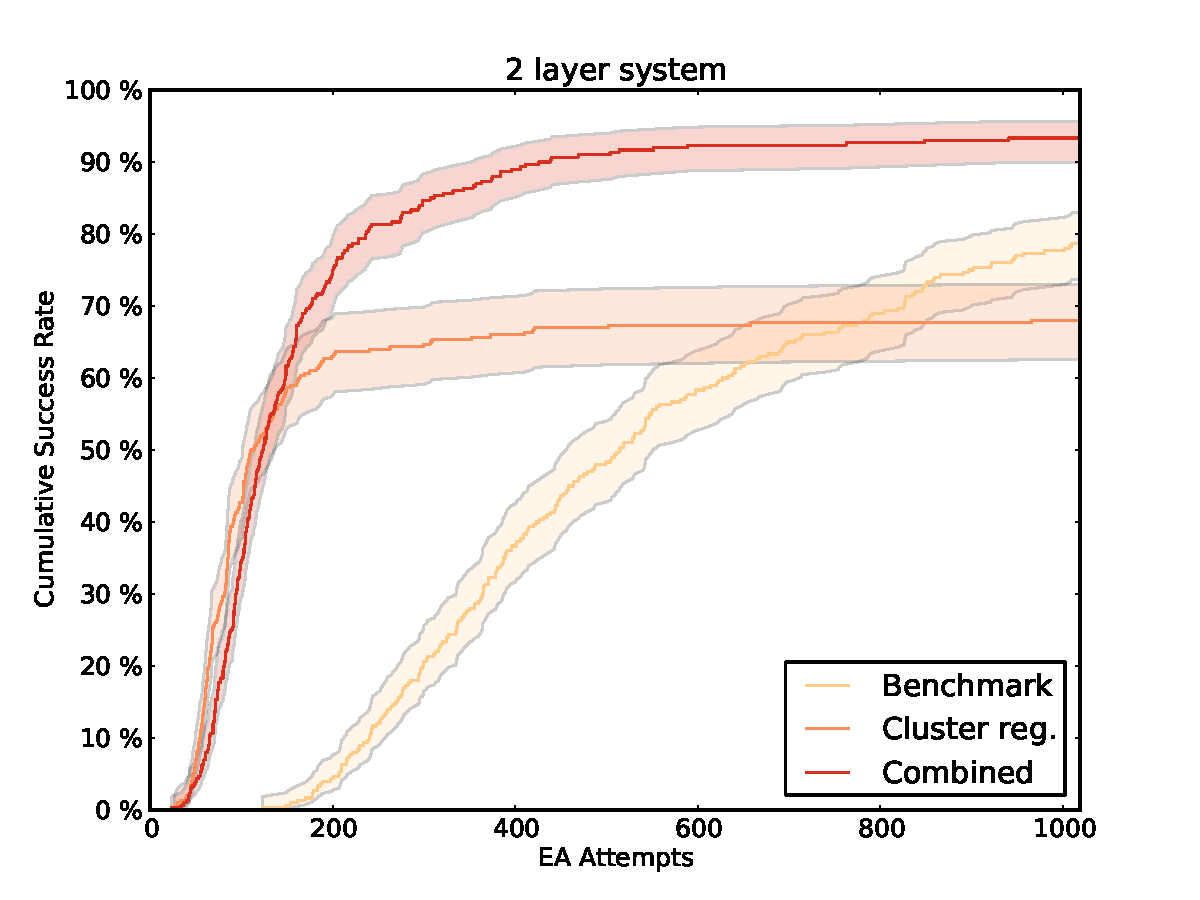
\includegraphics[width=1.0\columnwidth]{2lsuccess.pdf}
    \caption{Cumulative sussess for 2 layer system}
    \label{fig:fig4}
\end{figure}


\begin{figure}[h]
    \centering
    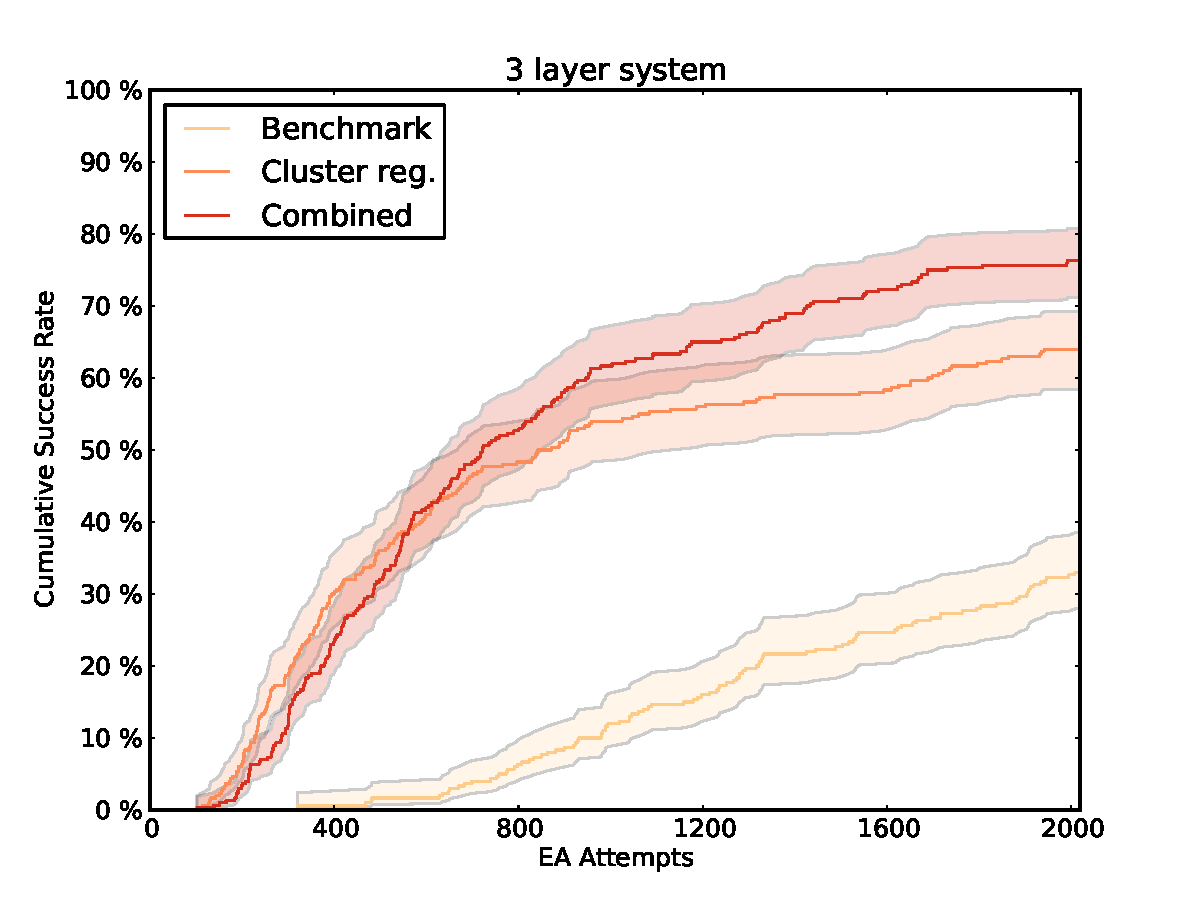
\includegraphics[width=1.0\columnwidth]{3lsuccess.pdf}
    \caption{Cumulative sussess for 3 layer system}
    \label{fig:fig5}
\end{figure}


\begin{figure}[h]
    \centering
    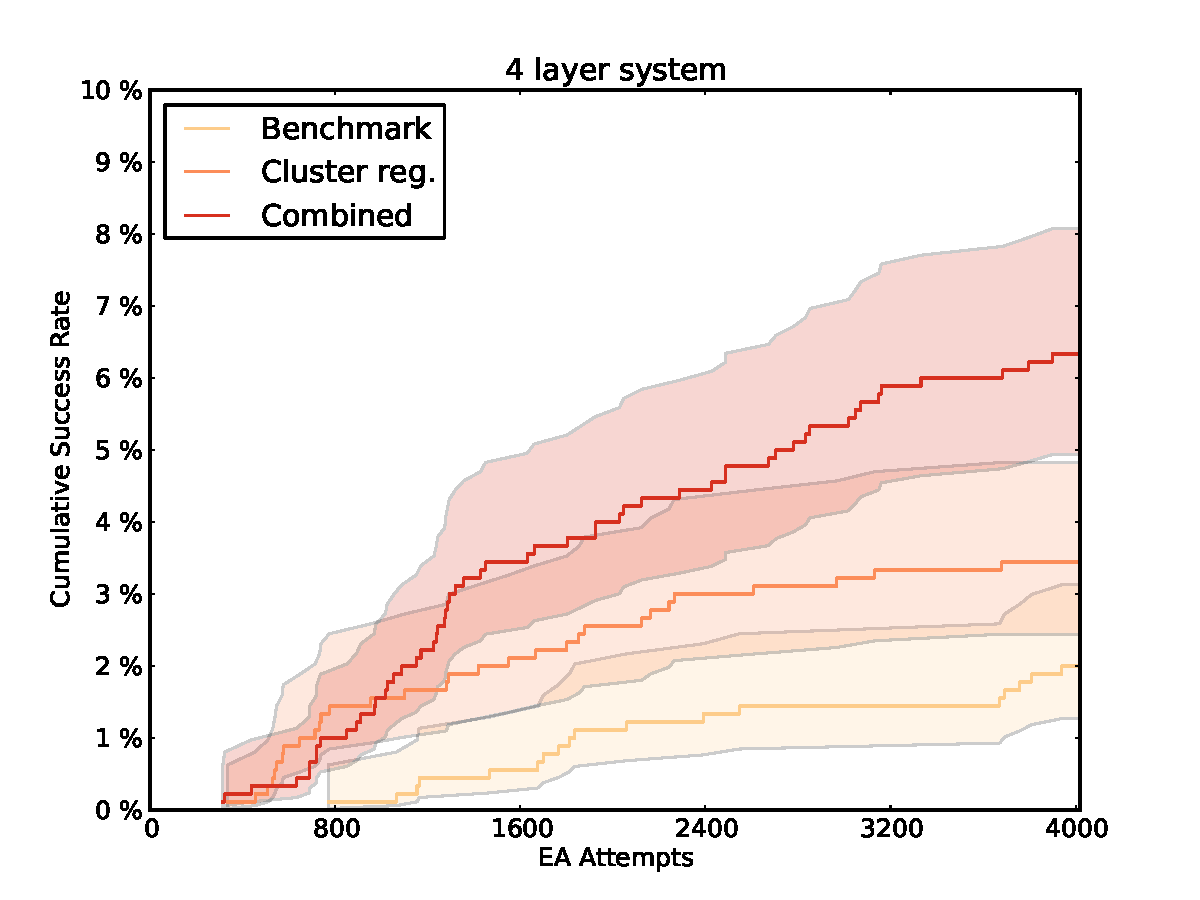
\includegraphics[width=1.0\columnwidth]{4lsuccess.pdf}
    \caption{Cumulative sussess for 4 layer system}
    \label{fig:fig6}
\end{figure}



We acknowledge support from the Danish Research Council (grant no. 0602-02566B) and from VILLUM FONDEN (Investigator grant, project no. 16562).

\begin{thebibliography}{12}  
  \bibitem{Starke1998} U. Starke \textit{et al}., Phys. Rev. Lett. \textbf{80}, 758 (1998).    
  \bibitem{Botu2015} {Adaptive Machine Learning Framework to Accelerate Ab Initio Molecular Dynamics.} V. Botu and R. Ramprasad, Int. J. Quantum Chem. 2015, 115 ,1075-18083. DOI:10.1002/qua.24836    
 \bibitem{Malay2009} {A Modified k-means Algorithm to Avoid Empty Clusters} Malay K. Pakhira, International Journal of Recent Trends in Engineering, Vol 1, No 1, May 2009
 \end{thebibliography}


\end{document}
